\documentclass[fleqn,usenatbib]{template/mnras}

%%% DEBUG SETTINGS - remove at the end %%%%%%%%%%%%%%%
\usepackage{silence} % silence error warinings
\WarningFilter{caption}{Unsupported document class} % caption doesn't know mnras..
\hbadness = 5000
\vbadness = 10000
% \usepackage{}

% MNRAS is set in Times font. If you don't have this installed (most LaTeX
% installations will be fine) or prefer the old Computer Modern fonts, comment
% out the following line
%\usepackage{newtxtext,newtxmath} % not yet supported on arxiv and uni computer
%\usepackage{txfonts}

% Depending on your LaTeX fonts installation, you might get better results with one of these:
%\usepackage{mathptmx}
%\usepackage{txfonts}

% Use vector fonts, so it zooms properly in on-screen viewing software
% Don't change these lines unless you know what you are doing
\usepackage[T1]{fontenc} % make sure font is supported
% \usepackage{ae,aecompl} %obsolete when using modern fonts
\usepackage[final]{microtype} % make sure font is supported
% and a suitable font
\usepackage{lmodern} % use a modern font with T1 support
%\usepackage{cm-super} % use a modern font with T1 support


%%%%% AUTHORS - PLACE YOUR OWN PACKAGES HERE %%%%%

% Only include extra packages if you really need them. Common packages are:
%\usepackage[dvipdfmx]{graphicx}	% Including figure files
\usepackage{graphicx} % Including figure files
%\usepackage[skip=0pt]{subcaption}
\usepackage{amsmath}	% Advanced maths commands
\usepackage{amssymb}	% Extra maths symbols
\usepackage{pifont}	% Extra maths symbols
%\usepackage{bmpsize}  % PS still needs this for correct bounding boxes?


% TODO stuff, comment out for final submit
\usepackage{todonotes} % as long as we are editing...
%\usepackage{showframe} % for debug
%\overfullrule=5pt      % show overfull boxes

% I disabled hyperlink in the cls und included it here because of bugs
\usepackage{hyperref}   % Hyperlinks
\hypersetup{colorlinks=true,linkcolor=blue,citecolor=blue,filecolor=blue,urlcolor=blue}

\newcommand*{\rot}{\rotatebox{90}}
\newcommand*{\OK}{\ding{51}}
\newcommand*{\NO}{\ding{55}}

\newcommand{\lenstitle}[1]{\noindent\textbf{#1} --}
\newcommand{\params}[3]{(\(\Theta_\text{E}:#1\), $\varepsilon:#2$, $\alpha_\varepsilon:#3$ )}

\newcommand{\asw}[1]{ASW000#1}
\newcommand{\sw}[1]{SW~#1}
\newcommand{\model}[1]{SL model~#1}

\newcommand{\figref}[1]{\ref{fig:#1}}

\newcommand{\Mstel}{M_{\rm stel}}
\newcommand{\Mhalo}{M_{\rm h}}
\newcommand{\haloindex}{\mathcal{H}}
\newcommand{\ER}{$\Theta_{\text{E}}$} % einstein radius


\def\pwidth{.32\linewidth}


\input img/model_assignment



\title[Lens models for Space Warps CFHTLS]{Models of lens candidates from
  Space Warps CFHTLS}

\author[K\"ung et al]{Rafael K\"ung,$^{1}$
Prasenjit Saha,$^{1}$
Ignacio Ferreras,$^{2}$
Elisabeth Baeten,$^{3}$
\newauthor
Jonathan Coles,$^{4}$
Claude Cornen,$^{3}$
Christine Macmillan,$^{3}$
Phil Marshall,$^{5}$ 
\newauthor
Anupreeta More,$^{6}$
Lucy Oswald$^{7}$
Aprajita Verma$^{8}$
and Julianne K. Wilcox$^{4}$
%
\\
%
$^{1}$Physik-Institut, University of Zurich, Winterthurerstrasse 190, 8057 Zurich, Switzerland\\
$^{2}$Mullard Space Science Laboratory, University College London, Holmbury St Mary, Dorking, Surrey RH5 6NT, UK\\
$^{3}$Zooniverse, c/o Astrophysics Department, University of Oxford, Oxford OX1 3RH, UK \\
%$^{4}$Exascale Research Computing Lab, Campus Teratec, 2 Rue de la Piquetterie, 91680 Bruyeres-le-Chatel, France\\
$^{4}$Physik-Department, Technische Universit\"at M\"unchen
James-Franck-Str.~1, 85748 Garching, Germany\\
$^{5}$Kavli Institute for Particle Astrophysics and Cosmology, Stanford University, 452 Lomita Mall, Stanford, CA 94035, USA\\
$^{6}$Kavli Institute for the Physics and Mathematics of the Universe, University of Tokyo, 5-1-5 Kashiwanoha, Kashiwa-shi 277-8583, Japan\\
$^{7}$Murray Edwards College, University of Cambridge, Cambridge CB3 0DF, UK\\
$^{8}$Sub-department of Astrophysics, University of Oxford, Denys Wilkinson Building, Keble Road, Oxford, OX1 3RH, UK\\
}



% These dates will be filled out by the publisher
% \date{Accepted XXX. Received YYY; in original form ZZZ}

% Enter the current year, for the copyright statements etc.
\pubyear{2016}

% Don't change these lines
\begin{document}
\label{firstpage}
\pagerange{\pageref{firstpage}--\pageref{lastpage}}
\maketitle

\begin{abstract}
We report modelling follow-up of recently-discovered
gravitational-lens candidates in the CFHT Legacy Survey.  Lens
modelling was done by a small group of specially-interested volunteers
from the Space~Warps citizen-science community who originally found
the candidate lenses.  Models are categorised according to seven
qualitative and quantitive points.  Also included are some
improvements to the modelling software used (SpaghettiLens),
and discussion of strategies for scaling to future surveys
with more and frequent discoveries.

The candidates successfully modelled are all galaxies, with inferred
lensing masses ranging from $\sim10^{11}M_\odot$ to $>10^{13}M_\odot$.
Stellar masses have also been estimated, using photometry from the
CFHTLS pipeline and stellar-population models.  A trend well-known
in nearby galaxies, that star-formation efficiency is maximal for
total masses of $\approx10^{12}M_\odot$ and reduces for both lower and
higher masses, is discernable also in these much more distant
galaxies.
\end{abstract}

\begin{keywords}
gravitational lensing: strong -- citizen science
\end{keywords}

\section{Introduction}

By coincidence, the typical escape velocity of massive galaxies is
such that $v_{\rm esc}^2/c^2$ is comparable to the apparent sizes of a
galaxies at cosmological distances.  This coincidence is fortunate,
because it makes the lensing deflection angle (which is $2v_{\rm
  esc}^2/c^2$) of distant galaxies comparable to their size on the
sky, and as a result, strong lensing by galaxies tends to produce
images that probe the dark halos of those galaxies.  This is
important, because while there is a general consensus that basic
mechanism of galaxy formation involve gravitational collapse,
fragmentation, and mergers of dark-matter clumps, into which gas fell,
cooling through radiative processes to form dense clouds and
eventually stars, there is much debate about the details \citep[for a
  summary, see][]{2012RAA....12..917S}.  In particular, the nature of
dark matter remains mysterious: most researchers take it to be a
collisionless non-relativistic fluid (cold dark matter or CDM) readily
studied by simulations \citep[for example, the influential millenium
  simulation by][]{2005Natur.435..629S}.  But other scenarios have
also been considered, such as a cold condensing boson fluid
\citep{2016ApJ...818...89S}, or dark matter particles with internal
degrees of freedom \citep{2010MNRAS.405...77S}, or not matter at all
but a modification of gravity \citep{2016PhRvL.117t1101M}.

All this motivates using galaxy lenses to study the mutual dynamics of
dark matter and gas in galaxies.  Several studies in recent years have
done so
\citep{2009ApJ...703L..51K,2011ApJ...740...97L,2012MNRAS.424..104L,
  2016MNRAS.459.3677L,2016MNRAS.456..870B} but it is desirable to
enlarge the samples from tens of lensing galaxies to thousands.  Doing
so requires both finding more lenses and also modelling their masses.
Recent searches through the CFHTLS \citep{2012SPIE.8448E..0MC} using
arc-finders
\citep[e.g.,][]{2012ApJ...749...38M,2014A&A...567A.111M,2014ApJ...785..144G}
by machine learning
\citep[e.g.,][]{2016A&A...592A..75P,2017arXiv170302642L} and by visual
inspection by citizen-science volunteers in Space~Warps
\citep{2016MNRAS.455.1191M} have, between them, discovered an average
of four lenses per square degree, so one can be optimistic about
finding many thousands of lenses in the next generation of wide-field
surveys, from the LSST in optical and the SKA in radio on the ground,
and Euclid and WFIRST in orbit.

The expected flood of new lens discoveries will need a similarly huge
modelling effort to reconstruct their mass distributions.  To prepare
for the challenge of massive-sample lens modelling,
\cite{2015MNRAS.447.2170K} developed a new modelling strategy,
implemented as the SpaghettiLens system.  The idea is to collaborate
with experienced members of the citizen-science community, who have
already participated in lens discovery through Space~Warps, as well as
several other projects involving astronomical data.  The system was
tested on a sample of simulated lenses from Space~Warps.

This paper continues by applying SpaghettiLens to lens-candidates
discovered through Space~Warps.  We present results from modelling of
56 of the 59 lens candidates reported by \cite{2016MNRAS.455.1191M}.
Each lens candidate was modelled in a collaborative refinement
process, where anyone interested can create a new model or modify an
existing model to try and make it better.\footnote{This is in contrast
  to the main Space~Warps project for discovering lenses, where
  volunteers in a crowd of $\gtrsim10^4$ make independent
  contributions.  Each person is presented with a random selection of
  survey-patches and invited to (in effect) vote on each.  The system
  estimates each volunteer's skill level according to test-patches
  interspersed with the real data, and weights their votes accordingly
  \citep{2016MNRAS.455.1171M}.  There is an active forum for
  volunteers, but since everyone is seeing different data samples with
  minimal overlap, the forum has little if any influence on votes.}
The result model represents a consensus among contributors, as to the
best that could be achieved with the available data and software.

We characterise each model with seven diagnostics, grouped into three 
categories, whose purpose is to help identify which systems are most probably 
lenses, and which ones are likely to be most rewarding for future follow-up 
observations. The diagnostics are as follows.

\begin{itemize}
\item First we have diagnostics based on morphology of the
  system.
  Section~\ref{sec:morph} and Figure~\ref{fig:splinput} explain.
\begin{itemize}
\item Whether the images are unblended.  Distinct unblended images are
  an advantage in modelling, but not essential.
\item Whether all images are discernible.  The topography of an
  arrival-time surface, as encoded by a spaghetti diagram, may require
  more images than are visible, in which case the modeller has to
  insert conjectural image positions.
\item Whether the lens is fairly isolated.
\item The image morphology concisely described: double or quads,
  further sub-categorised to indicate the elongation direction of the
  lensing mass.
\end{itemize}
\item Second we have mass models, covered in Section~\ref{sec:massmodels}.
\begin{itemize}
\item Whether the mass map is reasonable. Figure~\ref{fig:kappa}.
\item Whether the arrival-time surface and synthetic image are
  plausible.  In particular, additional images are implied in regions
  where they are not observed signal an unsatisfactory model.
  Figures~\ref{fig:arriv} and \ref{fig:synth} and \ref{fig:encl}.
\end{itemize}
\item Third, whether the implied lensing mass is plausible, given the
  photometric data of the lensing galaxy.  Section~\ref{sec:stellar-mass}
  explains how we compare the lensing mass with the mass in stars in
  the lensing galaxy.  We estimate the stellar mass by comparing
  galaxy magnitudes from the CFHTLS pipeline with the well-known
  stellar-population models of \cite{2003MNRAS.344.1000B}.  We then
  extrapolate the stellar mass to a halo mass using the
  abundance-matching prescription of \cite{2010ApJ...710..903M}.
  Naturally, the lensing mass must be more than the stellar mass but
  no more than the total halo mass.  We then introduce what we call a
  halo index ($\haloindex$) which gives an idea of how the lensing mass
  compares with these two constraints.  Figure~\ref{fig:stelmass}.
\end{itemize}

Section~\ref{sec:summary} summarises and tabulates the diagnostics in
Table~\ref{tab:models}.  Interpretation of the results is preliminary,
because the systems are candidates at this stage, not secure lenses.
Moreover the candidate-lens redshifts have large uncertainties, while
the candidate-source redshifts can only be guessed at present.
Nevertheless it is interesting to see what trends we can observe with
the already-available data.

There are three appendices devoted to various technical issues
relating to modelling.  \cite{2015MNRAS.447.2170K} tested the system
on simulated lenses and identified some areas for improvement.  In
\S~\ref{subsec:sourcefit} we introduce fitting of the brightness
profiles of the source.  This feature has not yet been included in
SpaghettiLens, but has been carried out in post-processing for a few
especially interesting candidates.  In \S~\ref{subsec:hires} we show
that making mass maps fine-grained in the central region relieves a
tendency in the earlier work for mass to be too shallow. Then in
\S~\ref{subsec:parameter} we consider the possibility of fitting a
parametric lens model to the model ensemble; so far we have only been
successful at extracting an Einstein radius.

The online supplement gives results for all the modelled systems generated
for all the lensing candidates.



% \input parts/spl


%%%%%%%%%%%%%%%%%%%%%%%%%%%%%%%%%%%%%%%%%%%%%%%%%%%%%%%%%%%%%%%%%%%%%%%
\section{Image morphology}
\label{sec:morph}

The main input of a modeller to the process is a markup of the
candidate lens system, which we call a spaghetti diagram.  This is a
sketch of the arrival-time surface from a point-like source, with
proposed locations of maxima, minima and saddle points, and an implied
time-ordering of the images.  Such information encodes a starting
proposal for the mass distribution.  A spaghetti diagram is thus a
completely abstract construction, and moreover it refers to a
simplified system with a point source.  However, spaghetti diagrams
are intuitive because they tend to resemble the form of lensed arcs
\citep[see Fig.3 of][]{2008MNRAS.383..857F}, and of course they are
simple to draw, and easy to vary and refine in an open collaborative
environment. This makes them very practical for non-professional lens
enthusiasts in the citizen-science community.  Details and tests are
given in \citet{2015MNRAS.447.2170K}.

We now discuss the diagnostics that can be taken from the process of
drawing the spaghetti diagram, even before detailed mass-modelling
takes place.  Fig.~\ref{fig:splinput} shows nine examples, each
consisting of a cutout of the \SW  image of a lens candidate,
marked up with a spaghetti diagram.
The volunteers are initially presented a square image with side
82\arcsec (440~pixels) in full size, but they have the
ability to zoom in individually.
The cutouts presented in Figs.~\ref{fig:splinput} to \ref{fig:kappa}
are rescaled during post-processing, relative to the outermost image.

All the examples shown in Fig.~\ref{fig:splinput} identify five locations:
the centre of the main lensing galaxy, which is also a maximum of the
arrival time surface (red dots); two minima (blue dots); and two
saddle points (green dots and also self-intersections of the curves).
Only two (\sw{05} and \sw{42}) of the nine systems, however, have five
distinct features in plausible locations.  In the other seven
examples, an arc is interpreted as a blend of three or four images.
This defines the `unblended images' diagnostic.  Note that this
characterisation could be different if the spaghetti diagram were 
different.  For example, \sw{28} has also been modelled with the arc on
the right interpreted as a single image, rather than as three images
as shown in the figure; for such a model, the `unblended images'
diagnostic would be true.

The second diagnostic checks whether all images are visible.  For example,
we see in \sw{58} at the top left of Fig.~\ref{fig:splinput} that an
image at the second minimum is conjectural and does not correspond to
any visible feature.

The third diagnostic tests whether the lens is isolated, or whether
other galaxies could contribute to the lensing.  For this, we do not
consider stars or other clearly foregound objects.  Additional
galaxies contributing to the lensing mass can be marked by the
volunteer alongside the spaghetti diagrams.  An example can be seen as
the grey dot and circle in the cutout with \sw{57} at the top right of
Fig.~\ref{fig:splinput}.  Objects marked in this way are modelled as
point masses.  Other possible contributors to lensing are galaxies or
groups that are not in the immediate vicinity of the lensed images,
yet massive enough to exert an influence. These are accounted for by
allowing a constant but adjustable external shear.

We remark that the lack of expected lensed images, or the presence of
blended images or perturbing galaxies do not imply that a given
candidate is unlikely to be a lens.  This means, rather, that the
models are more uncertain and perhaps could be more easily improved by
trying further variations in the markup.

The fourth diagnostic is based on the fact that the arrangement of
lensed images of a pointlike source through a non-circular
gravitational lens depends on the location of the source relative to
the long and short axes of the lens.  This dependence is quite robust
and independent of many other details of the lensing mass
distribution.  Sources close to being dead-centre behind a lens tend
to produce quads; sources at larger transverse distance tend to
produce doubles.  We denote these as Q and D, respectively, and add a
prefix to the Q systems, as follows: we write LQ if the source is
inferred as displaced along the long axis of the lens, SQ if displaced
along the short axis, IQ if inclined to both axes, CQ if only very little or
no displacement is evident.  Although the
unlensed source and its location are obviously not seen, the LQ, SQ, IQ and CQ
cases correspond to easily-seen image morphologies \citep[see,
  e.g.,][]{2003AJ....125.2769S}.
\begin{itemize}
\item The simplest is the LQ case: this creates a saddle point and two
  minima in an arc, with the second saddle point on the other side of
  the lensing galaxy, closer to the galaxy than the arc.  \sw{58}
  and \sw{28} in the upper row of Fig.~\ref{fig:splinput} are typical
  examples of LQ.  If the source were moved outwards along the short
  axis, the minimum-saddle-minimum set would merge into a single minimum,
  leaving a D system; the transition is known as a cusp catastrophe.
\item The middle row of Fig.~\ref{fig:splinput} shows three IQ
  systems: \sw{05}, \sw{42} and \sw{19}.  This type has a characteristic
  asymmetry, often with two images close together.  If the source
  were moved outwards, the minimum-saddle pair would merge and
  mutually cancel, leaving again a D system. This transition is known
  as a fold catastrophe.
\item The lower row of Fig.~\ref{fig:splinput} shows three SQ
  systems: \sw{09}, \sw{29} and \sw{02}. The failed model, \sw{57}, at top right
  may also belong to this category.  Here the images have a
  fairly symmetric arrangement with an arc and a counter-image on the
  other side, but the spaghetti diagram is completely asymmetric.  If
  the source were moved outwards along the long axis, the
  saddle-minimum-saddle set  would merge into a single saddle --- another
  form of cusp catastrophe.  SQ can be visually distinguished from LQ
  by the relative distances of the arc and the counter-image.  For
  SQ the arc is closer, for LQ the counter-image is closer.
\end{itemize}
CQ systems are often called `cross' or `Einstein-cross' systems; IQ
systems are sometimes called `folds', with `cusp' commonly used for
both SQ and LQ.  The labels `short-axis quad' and so on are not
standard in the literature, but the morphological classification they
express is familiar to experienced modellers.  Hence they can be
useful to researchers wishing to apply other modelling methods to the
same systems.



\section{Mass models}\label{sec:massmodels}

A SpaghettiLens model consists of a statistical ensemble of free-form
maps of the sky-projected mass distribution responsible for lensing.
  Photometric lens
redshifts are used; source redshifts are set to $z=2$ unless an
unambiguous photometric redshift is available.  The models can,
however, be trivially rescaled to use better redshift values, as and
when they become available.

A spaghetti diagram is read by a server-side numerical engine
\citep[GLASS, developed by][]{2014MNRAS.445.2181C} which then returns
a statistical ensemble of mass maps.  The mass maps are made up of
mass tiles and are free-form, except that they are required to be
concentrated around the identified lens centre.  They are also
required to reproduce the given image locations, parities and time
ordering exactly.  Graphical representations of the mass map and
arrival-time surface are returned to the user for review.  The user
can post these results on a forum, or discard them and try again.
Volunteers can start the modelling process afresh, or they can take an
existing model from the forum and modify its input spaghetti diagram
or its accompanying options, and thus obtain a revised model.

Alongside is a synthetic image produced by modelling.  In it, the
fitted lensed images are shown in colour, while the lensing galaxy and
extraneous objects have been reduced to grayscale.
(Figure~\figref{synthimg} in \S~\ref{subsec:sourcefit} shows a
synthetic image from another model of the same system.) These two
panels are qualitative and display no units, and moreover, the mutual
alignment of the two panels is only approximate.

Figures~\figref{SW58} and \figref{SW19} appear plausible lens
candidates.  Their morphology is similar to SW28, but the saddle-point
counterimage is not visible.  We consider these lenses plausible but
less convincing.

Figures~\figref{SW36} and \figref{SW57} are cases where modelling
failed.

\begin{enumerate}
\item The middle row shows contour maps from the model.  At middle
  left, we have the arrival-time surface.
\item At middle right we have the mass distribution in the usual
  dimensionless form $\kappa$.  Again, these two panels are mainly
  qualitative: both panels are spatially registered and centred on the
  density-peak of the lens, but no scales have been included.
\item The base row supplies spatial and mass scales.  The left panel
  shows the circularly-averaged $\kappa$ of the model ensemble, with
  increasing radius (in arcsec).  The four short vertical lines
  correspond to the minima and saddle points marked in the upper-left
  panel.  The effective Einstein radius \ER is also shown.  As the radius
  scale indicates SW05 is comparatively large lens on the
  sky.
\item 
\end{enumerate}




\section{Stellar and halo mass estimates}
\label{sec:stellar-mass}

The stellar masses of the lens galaxies are derived by comparison of
the photometric data with M/L estimates from population synthesis
models.  In principle, a detailed analysis of the spectral energy
distribution is needed to derive accurate stellar masses
\citep[e.g.][]{2009ApJS..185..253G,2011MNRAS.418.1587T}.  However,
estimates to within 0.3\,dex in $\log(\Mstel/\Msun)$ can be derived
with a single colour, preferably tracing a rest-frame colour similar
to $U-V$ \citep[see Fig.~1 of][]{2008MNRAS.383..857F}.  There is some
evidence from spectral lines that massive galaxies tend to have a more
bottom-heavy IMF than the Milky Way, but a much higher stellar
mass-to-light would over-predict the mass in some lensing systems
\citep{2015MNRAS.454L..71S}.

In this paper we further simplify the analysis by assuming a
relationship between the apparent total magnitude and stellar mass, at
the redshift of the lens.  For typical stellar-population parameters,
the variation of this relation is at most 1\,dex.  A further possible
systematic error is contamination of the light of the lensing galaxy
by the lensed background galaxy.  Reducing or eliminating the latter
would require detailed fitting of light distributions for each
candidate \citep[see][]{2011ApJ...740...97L}, which we have not yet
attempted.  Nonetheless, because the lensing masses range over two
order of magnitude, it is still interesting to compare with very rough
stellar masses.

We make use of the \citet{2003MNRAS.344.1000B} models to derive two
functional forms of the stellar mass with respect to SDSS-$i$ band
magnitudes. The models have solar metallicity, with a Chabrier IMF,
and assume two different age trends: a ``young'' model, with a
constant 500\,Myr age at all redshifts, and an ``old'' model where the
age is the oldest one possible at each redshift, adopting a standard
$\Lambda$CDM model with $H_0=70$\,km\,s$^{-1}$\,Mpc$^{-1}$ and
$\Omega_m=0.3$.

Figure~\ref{fig:stelmass} shows a comparison of stellar and lensing
masses.  The comparatively large span in the stellar mass shows the range 
between the masses derived using the two age trends respectively
and lies between 0.4 and 0.8~dex.
It will be improved in future work by using available optical and NIR 
magnitudes to derive more accurate constraints on the stellar populations.
In addition, we also derive halo masses for the lenses using an
abundance-matching formula.  This technique matches the distribution
function of observed stellar mass in galaxies with that of dark-halo
masses in $N$-body simulations to derive a simple relation between
stellar mass and halo mass.  We emphasize that a halo mass from
abundance matching should be considered an ``average'' estimate, and a
significant scatter can be expected as galaxies with the same stellar
mass can be found in different environments. We refer the reader to
\cite{2012MNRAS.424..104L} for an assessment of the effect of
abundance matching on the derivation of dark matter halo properties in
lensing galaxies. We follow the prescription of
\citet{2010ApJ...710..903M}, namely:
\begin{equation}
\begin{aligned}
\frac{\Mstel}{\Mhalo} &= \frac{2C_0}{(\Mhalo/M_1)^{-\beta} +
                                     (\Mhalo/M_1)^\gamma} \\
C_0 &= 0.02820, \quad M_1 = 10^{11.884} M_\odot \\
\beta &= 1.057, \quad \gamma = 0.556.
\end{aligned}
\end{equation}
Figure~\ref{fig:stelmass} may be compared with Figure~4 in
\cite{2011ApJ...734...69M}.

The comparison of lensing and stellar masses provides us with the last
of our model diagnostics.  This is a halo-matching index:
\begin{equation}
\haloindex = \frac{\ln(M/\Mstel)}{\ln(\Mhalo/\Mstel)}
\end{equation}
that relates the observed lensing to stellar mass, with the
global ratio expected if the host halo corresponds to the
average value derived by abundance matching. Several cases
for $\haloindex$ can be considered:
\begin{itemize}
\item $\haloindex < 0$ is unphysical because $M<\Mstel$.
\item $\haloindex = 0$ is when the stellar mass exactly accounts for the
  lensing mass.
\item $0 < \haloindex < 1$ is the typical situation, where the lens
  includes stars and dark matter, but not the full halo.
\item $\haloindex = 1$ means that the lens consists of the entire halo.
\item $\haloindex > 1$ is in tension with abundance-matching, because the
  lensing mass exceeds the expected halo mass.
\end{itemize}
The halo-matching index expresses whether the lensing mass is
plausible given the light from the candidate lensing galaxy.

Figure~\ref{fig:stelmass} and Table~\ref{tab:models} show most of the
candidates having stellar
and lensing mass typical of massive ellipticals\footnote{
  Exact values can be found in the online version of Table~\ref{tab:models}}.
SW05 is one of the
most massive of all the candidates, with a mass of galaxy-group scale.
It is a particularly attractive system for follow-up observations at
higher resolution, as it is a large system with clear multiple-image
features, and modelling leaves little doubt that it is a lens.  SW04
seems to be even more massive, but the diagnostics leave some doubts
about this model.  The two lowest-mass systems, SW19 and SW42, are
important if they are indeed lenses, as they would be low-mass lenses
dominated by dark matter.  All the modelled systems have reasonable
stellar-mass fractions, except for two cases where the stellar-mass
fraction is too low ($\haloindex > 1$): these are SW42 and
SW57.  In the case of SW57, the model has poor diagnostics and should
be discounted.  The model for SW42, on the other hand, is quite
convincing --- except for the high halo-matching index.  If SW42 turns
out not to be a lens, that would support the halo-matching index as an
effective criterion for filtering models.



\section{Discussion}\label{sec:summary}

This work follows up on lens candidates reported in
\cite{2016MNRAS.455.1191M} from citizen-science volunteers, with
modelling.  Volunteers role is collaborative.  No robotic competitors.

Table~\ref{tab:models} characterises each modelled system is
(i)~according to the image morphology and how clear or indistinct it
is, (ii)~whether the mass map and synthetic lensed image appear to be
plausible, and (iii)~how the model mass compares with the estimated
stellar and full-halo masses.  Missing rows are due to photometry data
not available.

Figure~\ref{fig:stelmass} summarises the properties of the lens
candidates.  Most appear to have stellar and total mass typical of
massive ellipticals.  SW05 is the most massive of all the candidates,
with a galaxy-group scale mass.  Two systems, SW19 and SW42 have low
mass; the lens models are not entirely satisfactory, but seems
plausible.  If these are lenses, they are very interesting.  In
particular SW42 could be the most dark-matter dominated lens known.


%%%%%%%%%%%%%%%%%%%%%%%%%%%%%%%%%%%%%%%%%%%%%%%%%%
%%%%%%%%%%%%%%%%%%%% REFERENCES %%%%%%%%%%%%%%%%%%
%%%%%%%%%%%%%%%%%%%%%%%%%%%%%%%%%%%%%%%%%%%%%%%%%%

\bibliographystyle{template/mnras}
\bibliography{bib/bibli}


%%%%%%%%%%%%%%%%%%%%%%%%%%%%%%%%%%%%%%%%%%%%%%%%%%
%%%%%%%%%%%%%%%%% APPENDICES %%%%%%%%%%%%%%%%%%%%%
%%%%%%%%%%%%%%%%%%%%%%%%%%%%%%%%%%%%%%%%%%%%%%%%%%

\clearpage

\def\pwidth{.32\linewidth}

\def\includeten#1#2{
\includegraphics[width=\pwidth]{#1ASW0007iwp_4XBJWT3COV#2}%
\includegraphics[width=\pwidth]{#1ASW0007xrs_JHC3J2HYV7#2}%
\includegraphics[width=\pwidth]{#1ASW0008pag_5SXGXQYY6V#2}\\
\includegraphics[width=\pwidth]{#1ASW0007k4r_N7LTELSYTM#2}%
\includegraphics[width=\pwidth]{#1ASW00096rm_4Q3YCEWGLN#2}%
\includegraphics[width=\pwidth]{#1ASW0001ld7_OS3CYAKLRT#2}\\
\includegraphics[width=\pwidth]{#1ASW0002asp_5EKMWWVJHL#2}%
\includegraphics[width=\pwidth]{#1ASW0008qsm_TOFS7JNGEK#2}%
\includegraphics[width=\pwidth]{#1ASW000619d_011489#2}\\
%\includegraphics[width=\pwidth]{#1ASW000096t_7IPP7LWVOF#2}%
}

\def\includezehn#1#2{
\includegraphics[width=\pwidth]{#1SW58_ASW0007iwp_4XBJWT3COV#2}%   L
\includegraphics[width=\pwidth]{#1SW28_ASW0007xrs_JHC3J2HYV7#2}%   L
\includegraphics[width=\pwidth]{#1SW57_ASW0008pag_5SXGXQYY6V#2}\\% X
\includegraphics[width=\pwidth]{#1SW05_ASW0007k4r_N7LTELSYTM#2}%   I
\includegraphics[width=\pwidth]{#1SW42_ASW00096rm_4Q3YCEWGLN#2}%   I
\includegraphics[width=\pwidth]{#1SW19_ASW0001ld7_OS3CYAKLRT#2}\\% I
\includegraphics[width=\pwidth]{#1SW09_ASW0002asp_5EKMWWVJHL#2}%   S
\includegraphics[width=\pwidth]{#1SW29_ASW0008qsm_TOFS7JNGEK#2}%   S
\includegraphics[width=\pwidth]{#1SW02_ASW000619d_011489#2}\\%     S
%\includegraphics[width=\pwidth]{#1SW36_ASW000096t_7IPP7LWVOF#2}%
}

\begin{figure*}
\includeten{spaghetti/}{_input}
\caption{Marked-up images. \label{fig:markedup}}
\end{figure*}

\begin{figure*}
\includezehn{img/arrival_spaghetti/}{_arrival_spaghetti}
\caption{\label{fig:arriv}}
\end{figure*}

\begin{figure*}
\includeten{img/nsynth/}{_nsynth}
\label{fig:synth}
\caption{}
\end{figure*}

\begin{figure*}
\includezehn{img/kappa_map/}{_kappa_map}
\caption{\label{fig:kappa}}
\end{figure*}

\begin{figure*}
\includezehn{img/kappa_encl/}{_kappa_encl}
\caption{}
\end{figure*}


\begin{figure*}
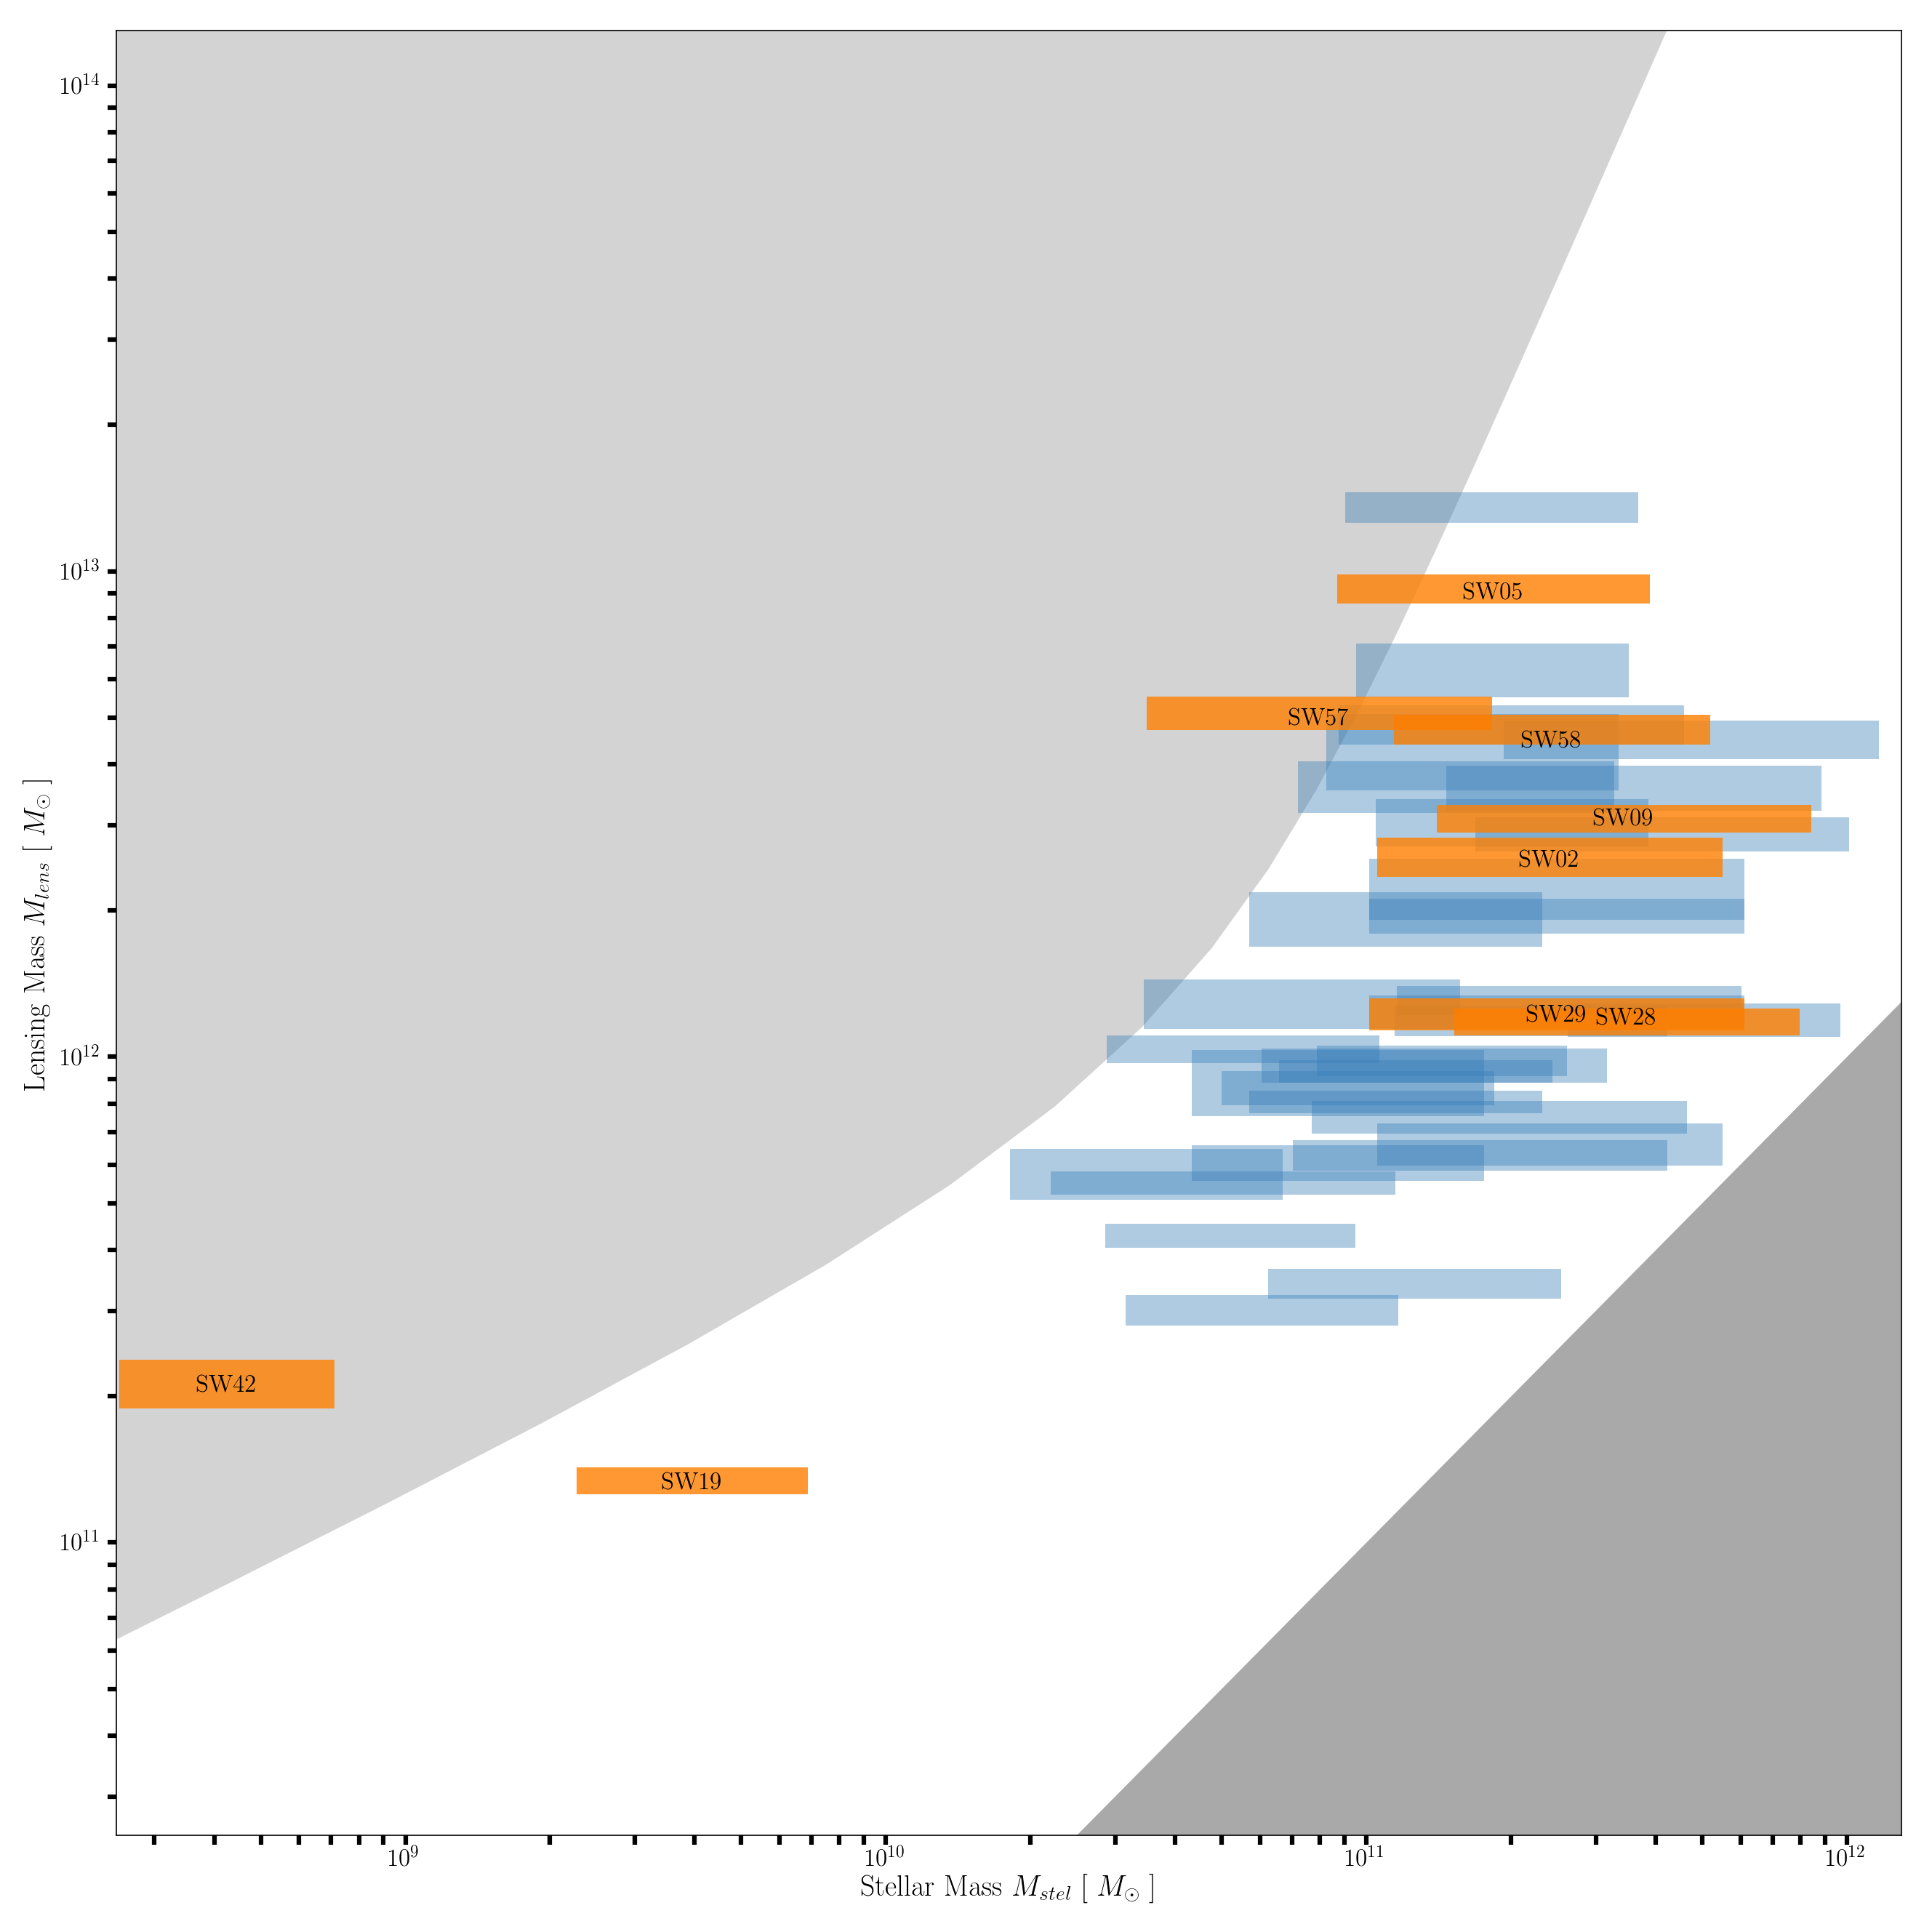
\includegraphics[width=\linewidth]{img/mlens_vs_mstel_one/mstel_vs_mtot_one}
\caption{Total mass in the model against the estimated stellar mass,
  alongside the values for the whole sample.  The lower-right shaded
  region is unphysical according to the stellar-population models,
  because it gives $M<\Mstel$. The upper-left shaded region is
  unphysical according to abundance matching, because it gives
  $M>\Mhalo$.  That is to say, the unshaded region is
  $0<\haloindex<1$. \label{fig:stelmass}}
\end{figure*}

\begin{table*}
  \caption{Categorisation of SW models}
  \label{tab:models}
  
\begin{tabular}{c c c | c c | c c c | c c c}
  \hline
  SWID & ASW id & model id
  
    & \rot{$z_\text{lens}$}

    & \rot{\shortstack[l]{image\\morphology}}
    
    & \multicolumn{1}{|l|}{\rot{\shortstack[l]{unblended\\images}}}
    & \rot{\shortstack[l]{all images\\discernible}}
    & \rot{\shortstack[l]{isolated\\ lens}}
    
    & \rot{\shortstack[l]{synthetic image\\ reasonable}}
    & \rot{\shortstack[l]{mass map\\ reasonable}}
    & \rot{\shortstack[l]{total vs stellar\\ mass ratio}}
  \\ \hline
  SW01 & ASW0004dv8 & J022409.5-105807 & 
    & 
    &  &  & 
    &  &  &  \\
    
  SW02 & ASW000619d & J140522.2+574333 & 0.7
    & LQ
    & \NO & \OK & \NO
    & \OK & \OK & 10 \\
    
  SW03 & ASW0006mea & J142603.2+511421 & 
    & 
    &  &  & 
    &  &  &  \\
    
  SW04 & ASW0009cjs & J142934.2+562541 & 0.5
    & CQ
    & \OK & \NO & \NO
    & \NO & \OK & 74 \\
    
  SW05 & ASW0007k4r & J143454.4+522850 & 0.6
    & IQ
    & \OK & \OK & \OK
    & \OK & \OK & 1.0e+02 \\
    
  SW06 & ASW0008swn & J143627.9+563832 & 0.5
    & LQ
    & \NO & \OK & \OK
    & \OK & \NO & 7 \\
    
  SW07 & ASW0007e08 & J220256.8+023432 & 
    & 
    &  &  & 
    &  &  &  \\
    
  SW08 & ASW00099ed & J020648.0-065639 & 0.8
    & D
    & \OK & \OK & \NO
    & \OK & \OK & 7 \\
    
  SW09 & ASW0002asp & J020832.1-043315 & 1.0
    & SQ
    & \NO & \OK & \OK
    & \OK & \OK & 9 \\
    
  SW10 & ASW0002bmc & J020848.2-042427 & 0.8
    & D
    & \OK & \NO & \OK
    & \NO & \NO & 3 \\
    
  SW11 & ASW0002qtn & J020849.8-050429 & 0.8
    & LQ
    & \NO & \OK & \NO
    & \OK & \OK & 3 \\
    
  SW12 & ASW0003wsu & J022406.1-062846 & 0.4
    & D
    & \OK & \OK & \NO
    & \OK & \OK & 4 \\
    
  SW13 & ASW00047ae & J022805.6-051733 & 0.4
    & LQ
    & \NO & \NO & \NO
    & \NO & \NO & 7 \\
    
  SW14 & ASW0004xjk & J023123.2-082535 & 
    & 
    &  &  & 
    &  &  &  \\
    
  SW15 & ASW0004nan & J084841.0-045237 & 0.3
    & LQ
    & \NO & \OK & \NO
    & \OK & \OK & 8 \\
    
  SW16 & ASW0009bp2 & J140030.2+574437 & 0.4
    & D
    & \NO & \NO & \OK
    & \NO & \OK & 5 \\
    
  SW17 & ASW0005rnb & J140622.9+520942 & 0.7
    & D
    & \OK & \NO & \NO
    & \NO & \OK & 6 \\
    
  SW18 & ASW0007hu2 & J143658.1+533807 & 0.7
    & D
    & \OK & \NO & \OK
    & \NO & \NO & 4 \\
    
  SW19 & ASW0001ld7 & J020642.0-095157 & 0.2
    & IQ
    & \NO & \OK & \NO
    & \NO & \OK & 34 \\
    
  SW20 & ASW0002dx7 & J021221.1-105251 & 0.3
    & IQ
    & \OK & \OK & \OK
    & \NO & \OK & 6 \\
    
  SW21 & ASW0004m3x & J022533.3-053204 & 0.5
    & D
    & \OK & \NO & \NO
    & \NO & \OK & 2 \\
    
  SW22 & ASW0009ab8 & J022716.4-105602 & 0.4
    & D
    &  & \NO & \NO
    & \NO & \OK & 2 \\
    
  SW23 & ASW0003r61 & J023008.6-054038 & 0.6
    & ???
    & ? & ? & ?
    & ? & ? & 23 \\
    
  SW24 & ASW00050sk & J023315.2-042243 & 0.7
    & LQ
    & \NO & \OK & \NO
    & \OK & \OK & 2 \\
    
  SW25 & ASW00007mq & J090308.2-043252 & 
    & 
    &  &  & 
    &  &  &  \\
    
  SW26 & ASW0005ma2 & J135755.8+571722 & 0.8
    & D
    & \OK & \NO & \OK
    & \NO & \NO & 9 \\
    
  SW27 & ASW0006jh5 & J141432.9+534004 & 0.7
    & LQ
    & \NO & \NO & \NO
    & \NO & \OK & 10 \\
    
  SW28 & ASW0007xrs & J143055.9+572431 & 0.7
    & LQ
    & \NO & \OK & \NO
    & \OK & \OK & 3 \\
    
  SW29 & ASW0008qsm & J143838.1+572647 & 0.8
    & SQ
    & \NO & \OK & \OK
    & \OK & \OK & 4 \\
    
  SW30 & ASW0002p8y & J021057.9-084450 & 
    & 
    &  &  & 
    &  &  &  \\
    
  SW31 & ASW00021r0 & J021514.6-092440 & 0.7
    & LQ
    & \NO & \OK & \NO
    & \OK & \OK & 24 \\
    
  SW32 & ASW0004iye & J022359.8-083651 & 
    & 
    &  &  & 
    &  &  &  \\
    
  SW33 & ASW0003s0m & J022745.2-062518 & 0.6
    & D
    & \OK & \OK & \NO
    & \NO & \OK & 17 \\
    
  SW34 & ASW00051ld & J023453.5-093032 & 0.5
    & ???
    & ? & ? & ?
    & ? & ? & 10 \\
    
  SW35 & ASW0004wgd & J084833.2-044051 & 0.8
    & LQ
    & \NO & \OK & \NO
    & \OK & \OK & 5 \\
    
  SW36 & ASW000096t & J090248.4-010232 & 0.4
    & D
    & \OK & \OK & \NO
    & \NO & \OK & 9 \\
    
  SW37 & ASW00086xq & J143100.2+564603 & 
    & 
    &  &  & 
    &  &  &  \\
    
  SW38 & ASW0009cp0 & J143353.6+542310 & 0.8
    & LQ
    & \NO & \OK & \OK
    & \OK & \OK & 9 \\
    
  SW39 & ASW0005qiz & J220215.2+012124 & 
    & 
    &  &  & 
    &  &  &  \\
    
  SW40 & ASW0008wmr & J221306.1+014708 & 
    & 
    &  &  & 
    &  &  &  \\
    
  SW41 & ASW0008xbu & J221519.7+005758 & 0.4
    & IQ
    & \OK & \NO & \OK
    & \OK & \OK & 16 \\
    
  SW42 & ASW00096rm & J221716.5+015826 & 0.1
    & IQ
    & \OK & \OK & \NO
    & \OK & \NO & 5.0e+02 \\
    
  SW43 & ASW0001c3j & J020810.7-040220 & 1.0
    & IQ
    & \NO & \NO & \NO
    & \NO & \OK & 6 \\
    
  SW44 & ASW0002k40 & J021021.5-093415 & 0.4
    & ???
    & ? & ? & ?
    & ? & ? & 34 \\
    
  SW45 & ASW00024id & J021225.2-085211 & 0.8
    & R
    & \NO & \OK & \OK
    & \NO & \OK & 8 \\
    
  SW46 & ASW00024q6 & J021317.6-084819 & 0.5
    & D
    & \OK & \OK & \NO
    & \OK & \OK & 6 \\
    
  SW47 & ASW0003r6c & J022843.0-063316 & 0.5
    & D
    & \OK & \NO & \OK
    & \NO & \OK & 26 \\
    
  SW48 & ASW0000g95 & J090219.0-053923 & 
    & 
    &  &  & 
    &  &  &  \\
    
  SW49 & ASW00007ls & J090319.4-040146 & 
    & 
    &  &  & 
    &  &  &  \\
    
  SW50 & ASW00008a0 & J090333.2-005829 & 
    & 
    &  &  & 
    &  &  &  \\
    
  SW51 & ASW0006e0o & J135724.8+561614 & 
    & 
    &  &  & 
    &  &  &  \\
    
  SW52 & ASW0006a07 & J140027.9+541028 & 
    & 
    &  &  & 
    &  &  &  \\
    
  SW53 & ASW00070vl & J141518.9+513915 & 0.4
    & D
    & \OK & \NO & \OK
    & \NO & \OK & 15 \\
    
  SW54 & ASW0007sez & J142620.8+561356 & 0.5
    & R
    & \NO & \OK & \NO
    & \OK & \OK & 16 \\
    
  SW55 & ASW0007t5y & J142652.8+560001 & 
    & 
    &  &  & 
    &  &  &  \\
    
  SW56 & ASW0007pga & J142843.5+543713 & 0.4
    & D
    & \OK & \NO & \OK
    & \NO & \NO & 18 \\
    
  SW57 & ASW0008pag & J143631.5+571131 & 0.7
    & LQ
    & \NO & \OK & \NO
    & \NO & \NO & 64 \\
    
  SW58 & ASW0007iwp & J143651.6+530705 & 0.6
    & SQ
    & \NO & \NO & \OK
    & \OK & \OK & 19 \\
    
  SW59 & ASW00085cp & J143950.6+544606 & 
    & 
    &  &  & 
    &  &  &  \\
    


  \hline

\end{tabular}

\end{table*}


\clearpage

\appendix

\section{Developments in SpaghettiLens}

\subsection{Improved synthetic images}\label{subsec:sourcefit}

The mass maps produced by current implementation of SpaghettiLens are
based on images of point-like features.  No information about extended
images is used, except in so far as they help the user identify images
of point-like features.  The synthetic images offered to users are
rudimentary, corresponding to conical light profiles (that is,
circular light profiles with brightness decreasing linearly with radius).

We have now developed a prototype of better way to generate synthetic
images.  Figure~\figref{synthimg} illustrates.  First, areas
containing lensed images are selected (green frames in the figure).
The selected areas should be as free as possible from of light from
the lensing galaxy or from extraneous objects.  Pixels within the
selected areas are mapped to a grid on the source plane, using bending
angles given by the mass model.  The mapping from lens-plane pixels to
source-plane grid cells is many-to-one, because of image multiplicity
and magnification.  The brightness of each source-plane pixel is set
to the mean of all the lens-plane pixels mapping to it.  Finally, the
mapping is run back to the lens plane.  The result is a synthetic
image.  In effect, one is reconstructing a source-plane brightness map
by least-squares.

The procedure is not yet implemented in SpaghettiLens but can be
applied in post-processing.  The new synthetic images could be used to
improve the mass reconstruction, by weighting the ensemble of maps
according to how good the synthetic images are, but we have not
attempted to do so as yet.

\begin{figure}
  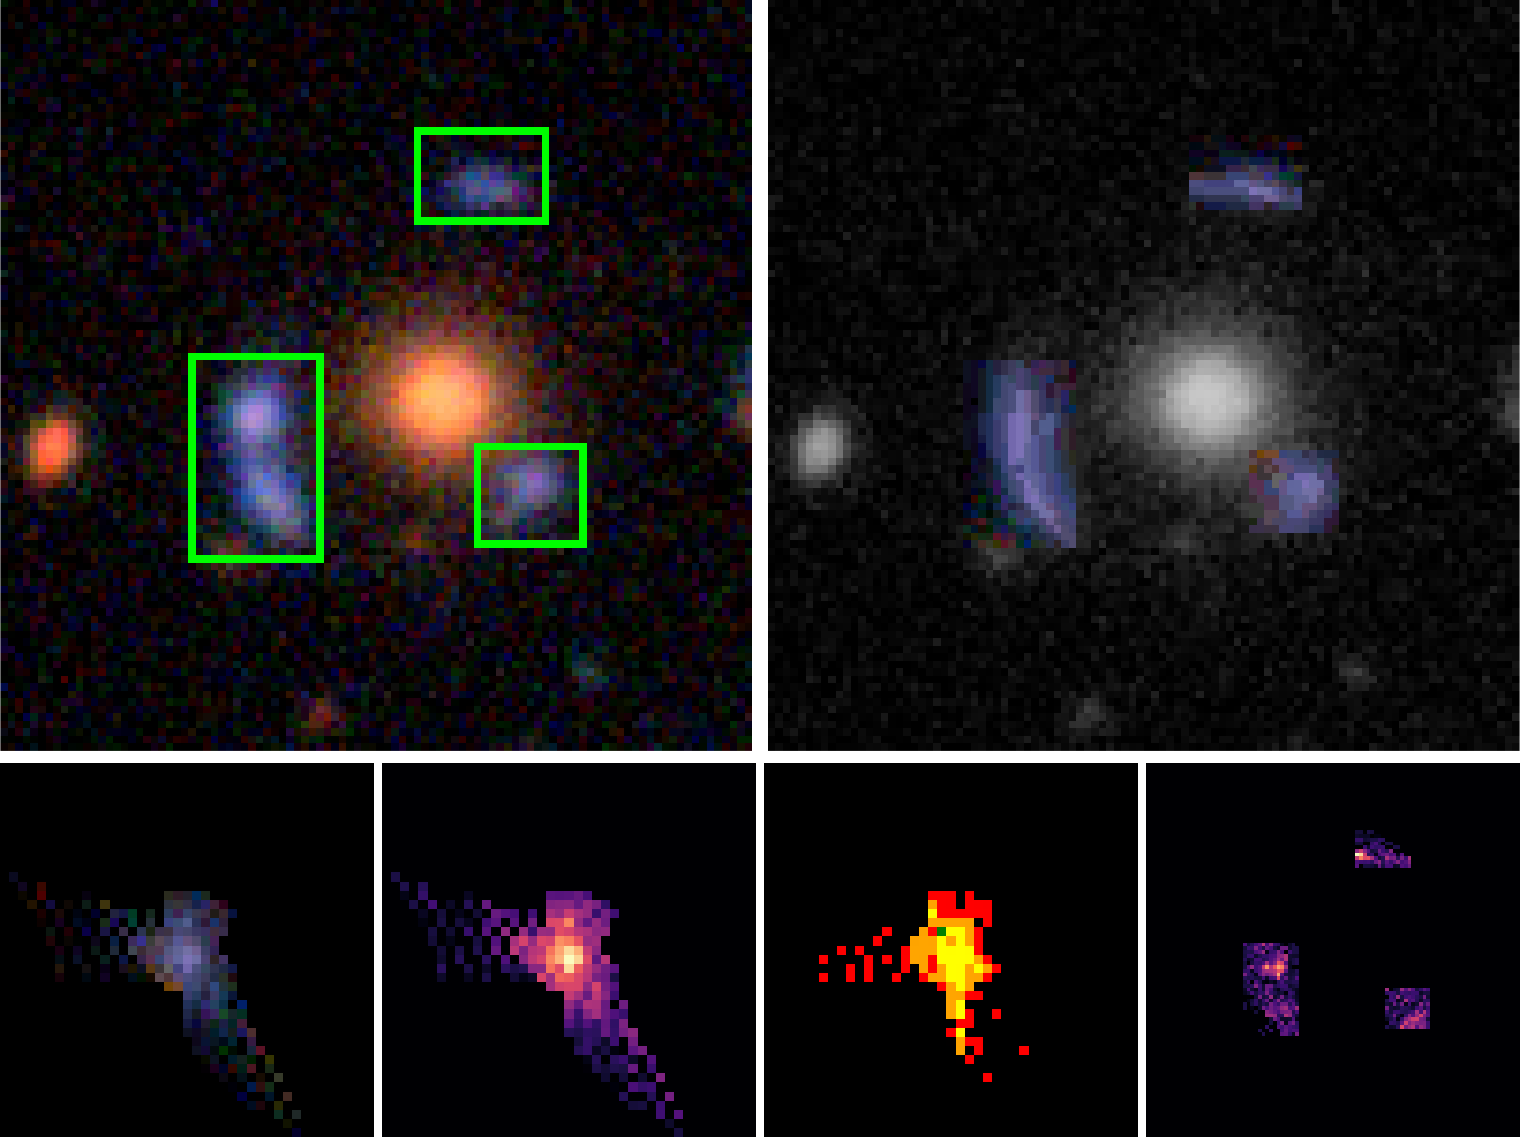
\includegraphics[width=\linewidth]{img/new_synth_img_detailed}
  \caption{Synthetic lensed image with source-profile fitting in SW05
    (J143454.4+522850). Top-left: original image, with areas
    containing lensed images enclosed within green frames.  Top-right:
    synthetic image (coloured arcs) with lensing galaxy and unrelated
    objects in greyscale.  Bottom from left to right: reconstructed
    source in colour, intensity (greyscale), count of lens plane
    pixels per source plane pixel, residual of original image to
    synthetic image.}
  \label{fig:synthimg}
\end{figure}

\subsection{Sub-sampling of central region}\label{subsec:hires}

The models of simulated lenses in \cite{2015MNRAS.447.2170K} showed a
tendency to be too shallow.  Allowing smaller mass tiles in the
central region, thus allowing the mass profile to rise more steeply
near the centre, was suggested as a possible cure.

Figure~\figref{subsampling} shows an experiment with smaller mass
tiles in the inner region.  Replacing the very central mass tile with
9 smaller tiles allows for steeper central profiles.  Doing the same
for the 25 innermost mass tiles allows for still steeper central
profiles, eliminating the systematic shallowness.  This is, however,
still not a completely satisfactory solution, because (a)~it increases
the number of mass tiles by 40\% and significantly increases the
computational time, and (b)~the square boundary between area with
different tile sizes is rather undesirable.
% 689 / 489 = 1.40899; in practice, runtime is more like x4 - x5!
% runtimes from logfiles: 87/22, 86/21, 85/16
The main modelling work in this paper was, however, done before the
experiments with smaller mass tiles was complete.  Some of the models
presented in this paper apply the intermediate option (corresponding
to the middle panel in Figure~\figref{subsampling}) while others use
the old system.  The results in this paper, however, mainly concern
the enclosed mass in the outer regions, so shallowness in the central
region should be inconsequential.

\begin{figure}
  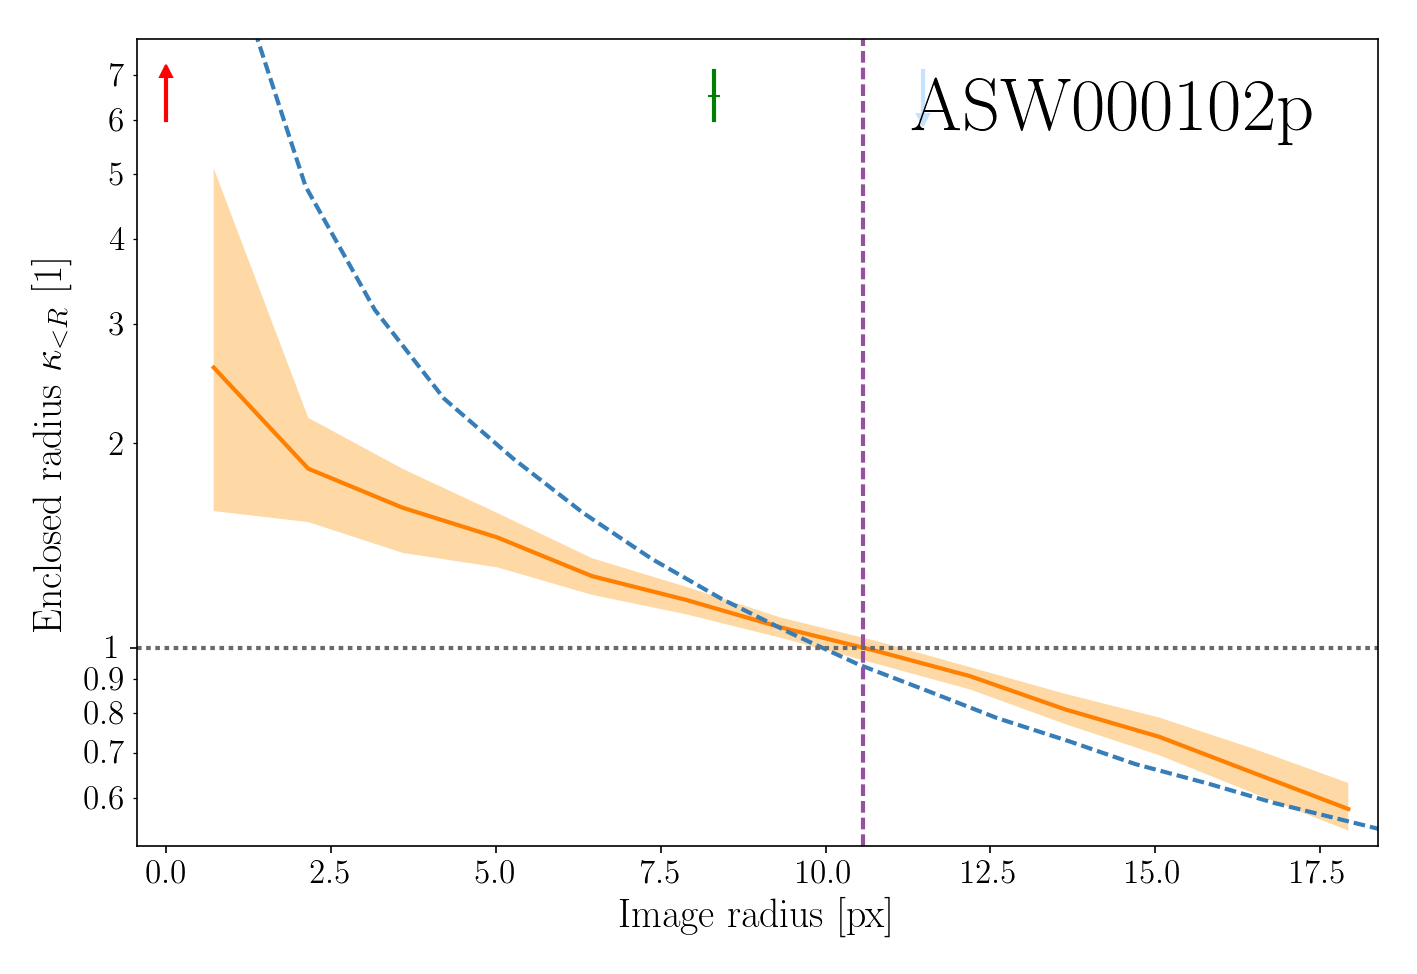
\includegraphics[width=.9\linewidth]{img/hires_comparison/ASW000102p_6941_11_hires_comparison}
  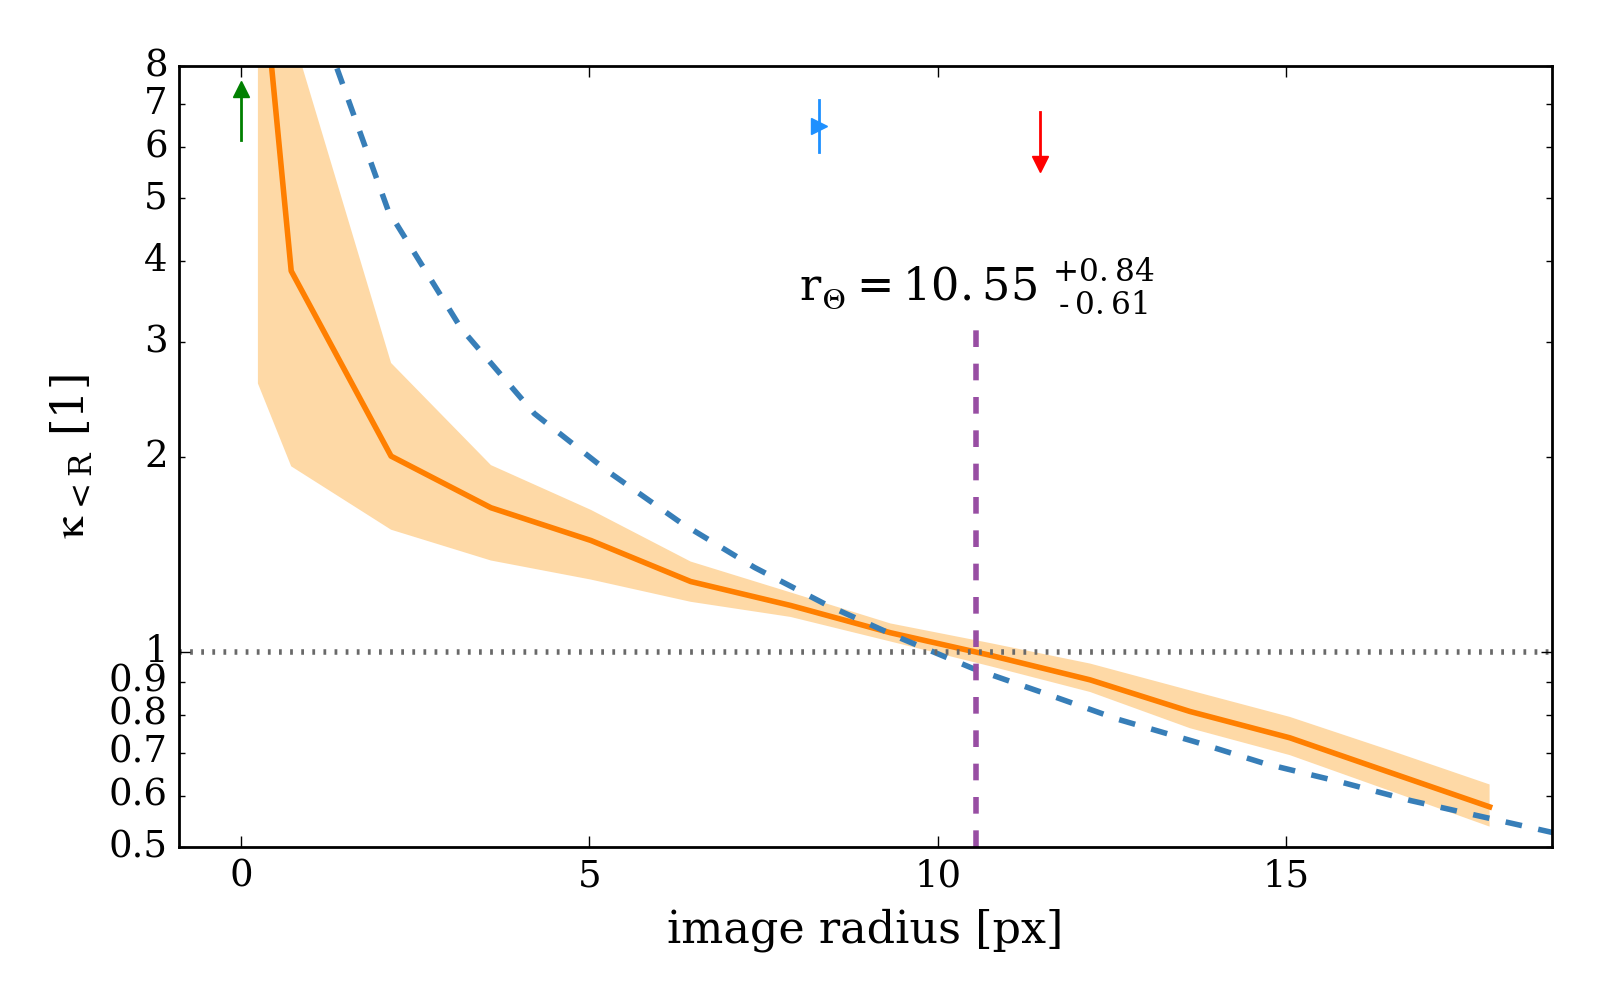
\includegraphics[width=.9\linewidth]{img/hires_comparison/ASW000102p_6941_13_hires_comparison}
  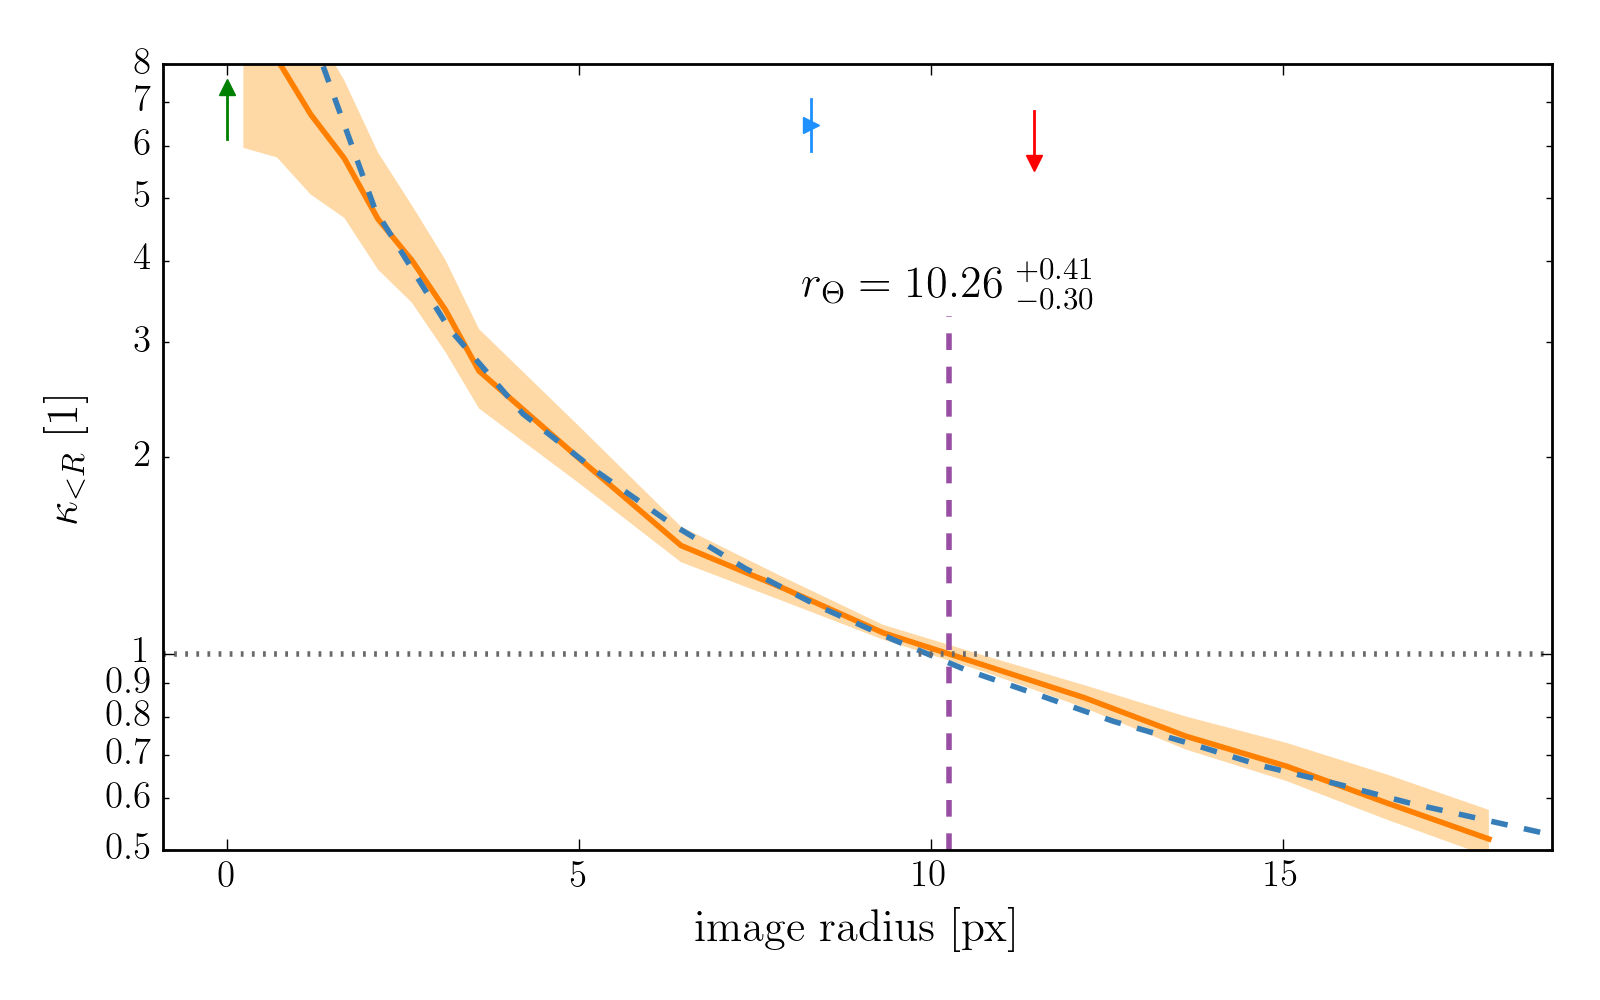
\includegraphics[width=.9\linewidth]{img/hires_comparison/ASW000102p_6941_33_hires_comparison}
  \caption{Model improvement resulting from using smaller mass tiles
    in the inner region of the mass model.  Shown here are the average
    enclosed $\kappa$ within a given projected radius, for three
    different reconstructions of a simulated lens (sim) from
    Space~Warps.  In each panel, the dashed blue curve is the correct
    answer.  The orange band represents the statistical ensemble from
    SpaghettiLens, the orange line being the ensemble mean.  Locations of
    images (maximum, saddle point, minimum) are marked with vertical
    arrows.  Crossing the horizontal $\kappa=1$ line is the effective
    Einstein radius \ER. The upper panel is from
    K\"ung et al., (2015) (see Figure~3 of that paper).  The middle
    panel is the result when the innermost mass tile is replaced by 9
    smaller tiles.  The lower panel results from replacing each of the
    innermost 5 by 5 tiles each with 9 smaller tiles.}
  \label{fig:subsampling}
\end{figure}

\subsection{Parameterisation of pixel models} \label{subsec:parameter}

In order to fit the set of pixelated models to a single parameterised model, a program was written that took a parameterised function and subtracted from it the mean and the principal components of the data, which were calculated using classical Principal Component Analysis.
This created the residuals function.
The number of components used in the analysis was varied, to test how this affected the output, and it was found that using 5 principle components tended to give a reasonable approximation.
A masking function was added which selected only the data points that fell inside the image of the lens, and the principal components were clipped in order to keep the values inside the region of the ensemble of models.
Any value higher than the clip was set to be the clip value.
This was chosen to be 2.5 as, assuming that the data follows a Gaussian error distribution, almost all the values for the variance should lie between 2 and 3 standard deviations from the mean.
Minimising the residuals function produces the set of parameters that fit the parameterised function to the original pixelated ensemble most closely.
A least squares fit was used to perform this minimisation.
The parameterised model function was obtained from the gravitational potential of an isothermal ellipsoid mass distribution \citep{2001astro.ph..2341K}.
This model is frequently used to describe gravitational lenses as it tends to fit well with observations.
The isothermal ellipsoid model outputs three useful parameters: the radius of the Einstein ring, the ellipticity of the model and the angle of the ellipticity from the vertical, giving the orientation of the galaxy.
By applying this model to simulated lenses for which the values of these parameters were already known, it was possible to gain an estimate of the projected accuracy of the results, before applying the model to the candidate lensing galaxies.

Preliminary results on recovery of Einstein radii are shown in
Figure~\ref{fig:parameter}.

\begin{figure}
  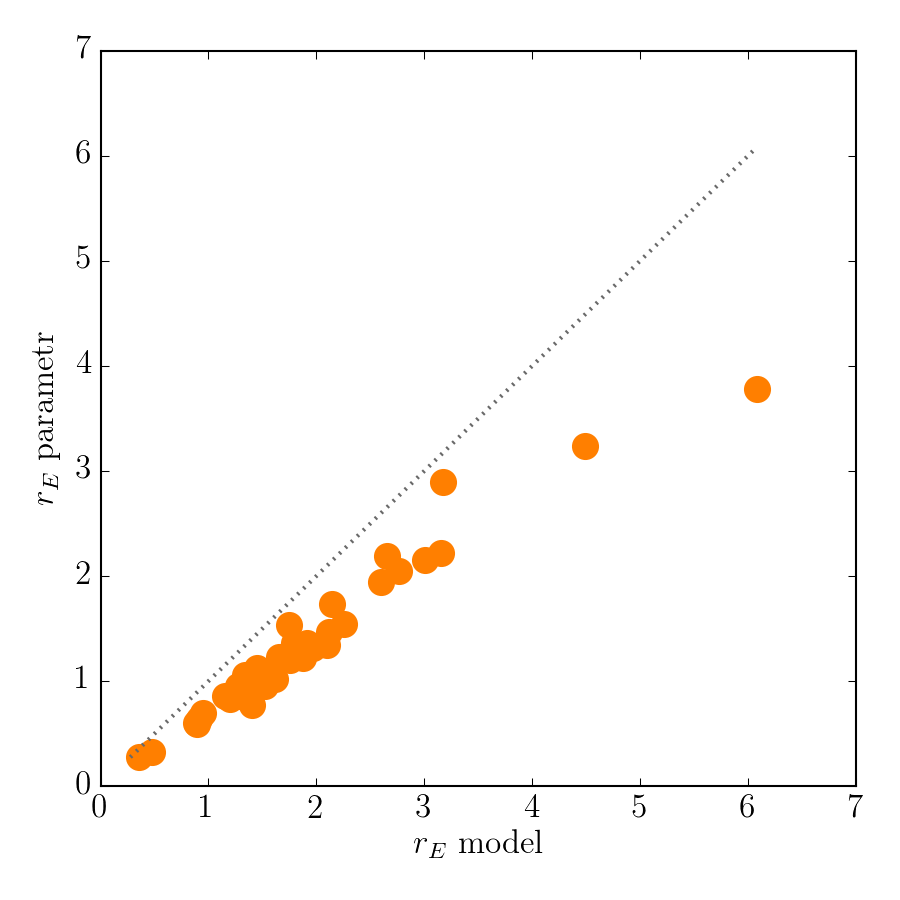
\includegraphics[width=\linewidth]{img/rE_comp/rE_comp.png}
  \caption{
    Comparison of Einstein radii \ER obtained from mass tiles directly to those obtained from a parameterized model to test the performance of the parametrisation algorythm.
    The parameterized model was generated using princible componant analysis on the ensemble of models.
    The blue dashed line represents a perfect recovery of \ER.
    }
  \label{fig:parameter}
\end{figure}





%\section{TODO}
%\listoftodos

% Don't change these lines
\bsp	% typesetting comment
\label{lastpage}
\end{document}

